\documentclass[11pt, a4paper, oneside]{report}
\usepackage{acronym}
\usepackage[hidelinks]{hyperref}
\usepackage{subcaption}
\usepackage{float}
\usepackage[utf8]{inputenc}
\usepackage{graphicx}
\graphicspath{{./img/}}
\usepackage{url}
\usepackage{enumerate}
\usepackage{enumitem}
\usepackage[style=numeric,sorting=none,backend=biber, doi=false, isbn=false,eprint=false]{biblatex}
\addbibresource{bibl.bib}
\usepackage[english]{babel}
%%page layout
\usepackage[a4paper, left=30mm, right=30mm, top=25mm, bottom=25mm,includehead,includefoot,heightrounded]{geometry}

% text formatting
\usepackage{ragged2e}
\usepackage{setspace}
\righthyphenmin=62
\lefthyphenmin=62

%include pdf with title page
\usepackage{pdfpages}

%use arial font
\usepackage[T1]{fontenc}
\usepackage{helvet}
\renewcommand{\familydefault}{\sfdefault}

%header
\usepackage{titlesec}
\usepackage{parskip}
\usepackage{fancyhdr}

\fancyhead{}
\fancyhead[L]{\includegraphics[scale=0.45]{UPM_logo.png}}
\fancyhead[R]{\includegraphics[scale=1]{UPM_logo1.png}}
\renewcommand{\headrulewidth}{0pt}
\fancyfoot{}
\fancyfoot[R]{\thepage}
\renewcommand{\footrulewidth}{0pt}

\fancypagestyle{plain}{%
    \fancyhf{} % clear all header and footer fields
    \fancyhead[L]{
\includegraphics[scale=0.05]{upm_logo.png}}
    \fancyhead[R]{
\includegraphics[scale=0.65]{etsist_logo.jpg}}
    \fancyfoot[R]{\thepage}
    \renewcommand{\footrulewidth}{0pt}
}
\fancypagestyle{infotext}{%
    \fancyhf{}
}

% Set the proper format for the headers
\titleformat{\chapter}[display]
  {\normalfont\sffamily\huge\bfseries}
  {\chaptertitlename\ \thechapter}{20pt}{\Huge}
\titleformat{\section}
  {\normalfont\sffamily\Large\bfseries}
  {\thesection}{1em}{}
\titleformat{\subsection}
  {\normalfont\sffamily\large\bfseries}
  {\thesubsection}{1em}{}
  
\title{{\LARGE UNIVERSIDAD POLITÉCNICA\\ DE MADRID}\\
\vskip 5mm
{\large \textbf{ESCUELA TÉCNICA SUPERIOR DE INGENERÍA\\
Y SYSTEMAS DE TELECOMUNICACIÓN}}\\
\vskip 5mm
{\large MSc in Systems and Services Engineering for the Information Society}\\
\vskip 10mm
{
\includegraphics[]{upm_only_logo.png}}\\
\vskip 5mm
{\textbf{Dataflow Specification of a K-Means Clustering Algorithm}}\\
\vskip 10mm
{Master Thesis}}
\author{Marta Rodríguez Ramos}
\vskip 40mm
\date{Madrid, October 2019}

\pagestyle{plain}

\linespread{1.05}

%\usepackage{xargs}                      % Use more than one optional parameter in a new commands
%\usepackage[pdftex,dvipsnames]{xcolor}  % Coloured text etc.
%%
\begin{document}
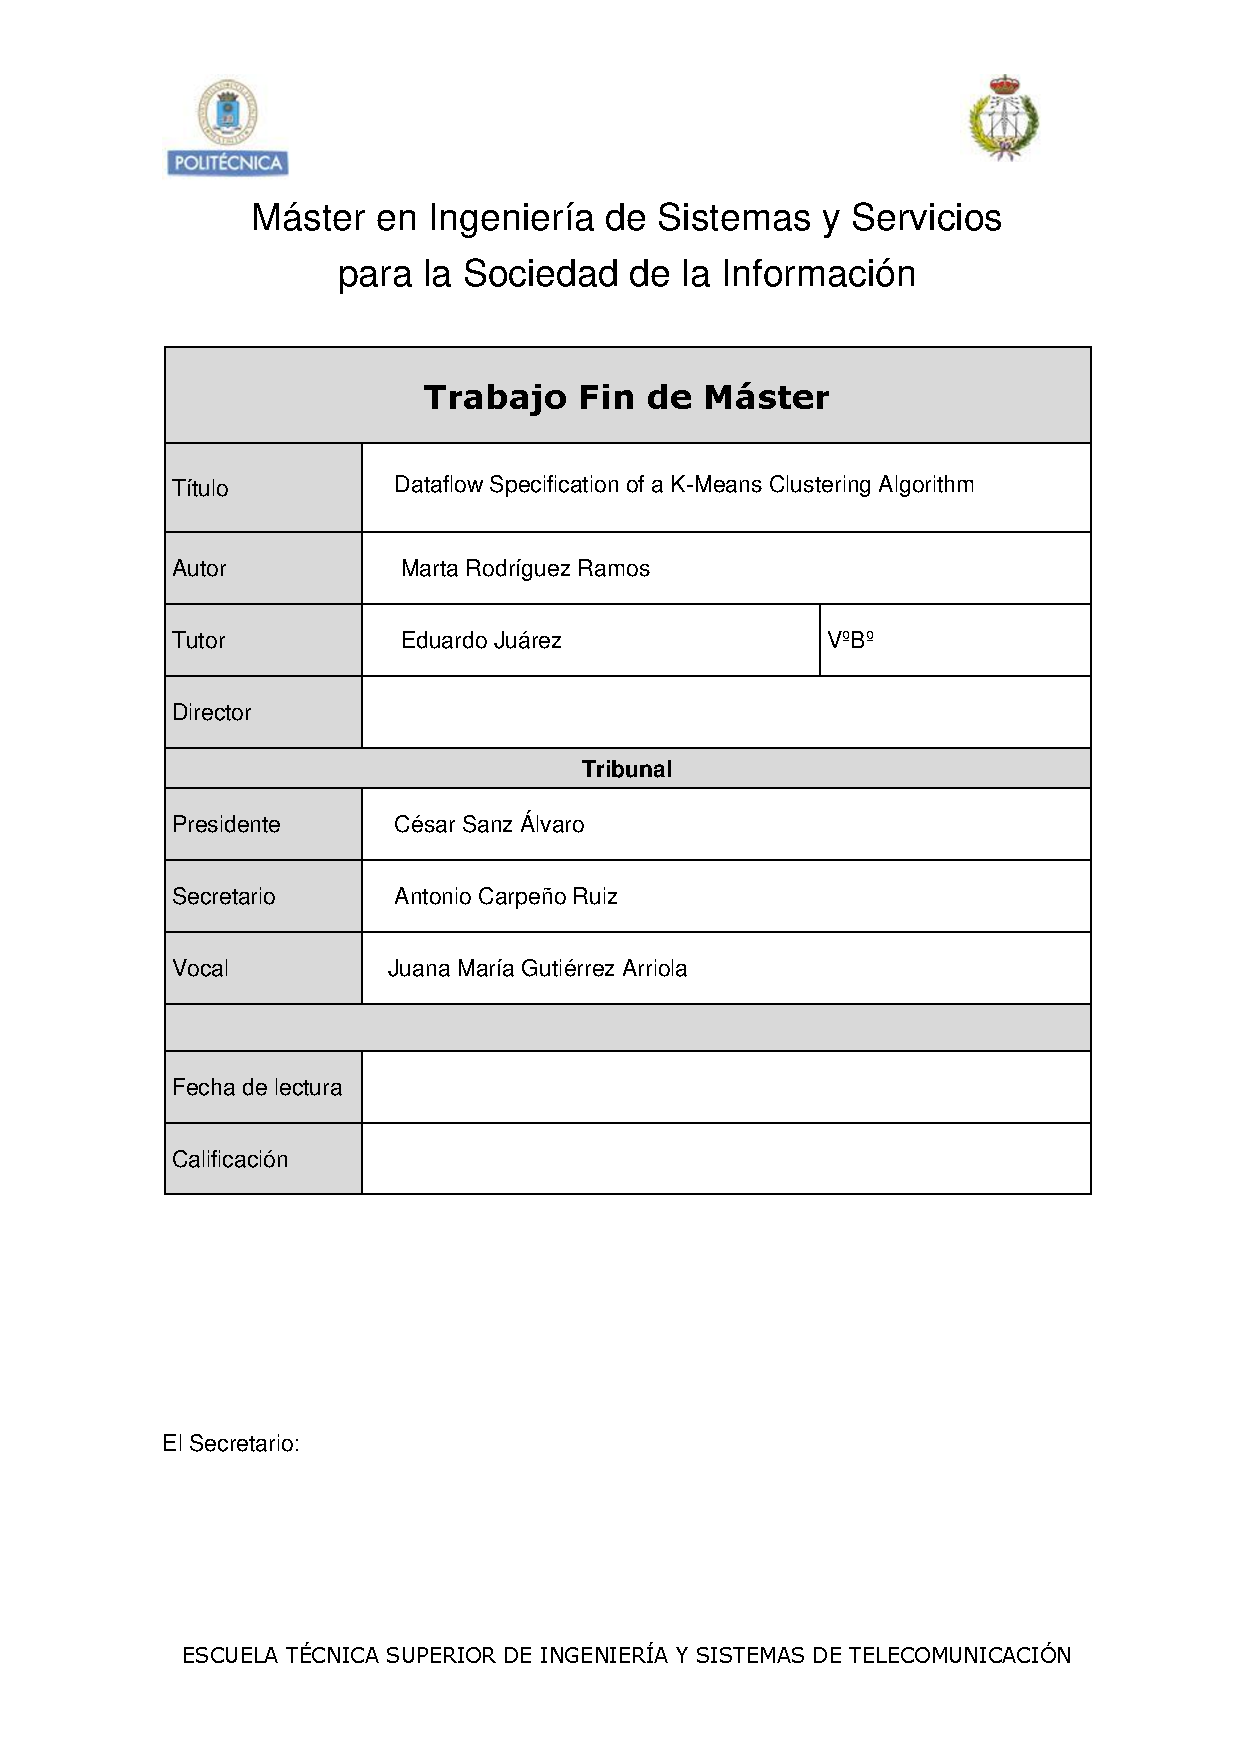
\includepdf[pages=-]{first_page.pdf}
\sloppy
\maketitle\thispagestyle{empty}
\newgeometry{left=30mm, right=30mm, top=25mm, bottom=25mm,includehead,includefoot,heightrounded, headheight=54pt}
\pagenumbering{roman}
\tableofcontents
\listoffigures
\listoftables
\chapter*{List of Acronyms}
	\begin{acronym}
\acro{6LoWPAN}{IPv6 over Low-Power Wireless Personal Area Networks}
\acro{ACK}{Acknowledge}
\acro{ACL}{Access Control List}
\acro{API}{Application Programming Interface}
\acro{CoaP}{Constrained Application Protocol}
\acro{CoaPS}{DTLS-Secured Constrained Application Protocol}
\acro{DTLS}{Datagram Transport Layer Security}
\acro{DDoS}{Distributed Denial of Service}
\acro{EUI}{Extended Unique Identifier}
\acro{FS}{File System}
\acro{GPU}{Graphics Processing Unit}
\acro{Hops}{Hadoop Open Platform-as-a-Service}
\acro{HDFS}{Hadoop Distributed File System}
\acro{HTTP}{Hypertext Transfer Protocol}
\acro{HTTPS}{Hypertext Transfer Protocol Secure}
\acro{IMEI}{International Mobile Equipment Identity}
\acro{IP}{Internet Protocol}
\acro{IPSO}{Internet Protocol for Smart Objects}
\acro{IoT}{Internet of Things}
\acro{JDBC}{Java Database Connectivity}
\acro{JSON}{JavaScript Object Notation}
\acro{JVM}{Java Virtual Machine}
\acro{JWT}{JSON Web Token}
\acro{MAC}{Media Access Control}
\acro{ML}{Machine Learning}
\acro{MVC}{model-view-controller}
\acro{MVVM}{model-view-viewmodel}
\acro{NAT}{Network Address Translation}
\acro{OMA LwM2M}{Open Mobile Alliance Lightweight Machine-to-Machine}
\acro{PKI}{Public Key Infrastructure}
\acro{PSK}{Pre-Shared Key}
\acro{REST}{Representational State Transfer}
\acro{RPK}{Raw Public Key}
\acro{SQL}{Structured Query Language}
\acro{TLS}{Transport Layer Security}
\acro{TSDB}{Time-Series Database}
\acro{UI}{User Interface}
\acro{URN}{Uniform Resource Name}
\acro{UUID}{Universally Unique Identifier}
\acro{VM}{Virtual Machine}
\end{acronym}
\onehalfspacing
\righthyphenmin=62
\lefthyphenmin=62
\justify
\chapter*{Abstract}
	In the 21st century, artificial intelligence has shown an upward trend of growth as one of the most important area in computer science. Furthermore, this field has had a high social impact on medicine providing real-time medical diagnoses through image processing and clinical trials. 

The present research work is developed within the context of HELICoiD. Furthermore, HELICoiD project exploits hyperspectral images as they are used along with machine learning for detecting and delineating tumours in brain tissues through a processing toolchain. This toolchain consists of supervised as well as unsupervised methods. 

The accurate delimitation of brain cancer is an important task having a surgery. Several techniques are used in order to guide neurosurgeons in the removal of the tumour.In this approach, the K-Means clustering algorithm aims at the accurate delimitation of the tumour borders. 

The implementation of this algorithm is performed using a dataflow specification tool called PREESM. This tool uses the Parameterized and Interfaced Synchronous Dataflow ($\pi SDF$) MoC model which is a hierarchical and dynamically reconfigurable extension of the SDF MoC. This model is known for their analyzability, their predictability and their natural expressivity of task parallelism in signal processing algorithms. The objective of parallelizing this algorithm is to speed up computations for data clustering to target real time response.In order to achieve this objective, the atomic operations which consume most of the execution time are firstly parallelized.

The results achieved are accurately analysed and validated using an in-vivo hyperspectral human brain image database. Experimental results illustrates that the PREESM version can reach speed-up of    than the secuantial's implementation one. Up to our knowledge, the work done in this thesis approaches real time during surgery as possible.


\chapter*{Resumen}
	En el siglo XXI, la inteligencia artificial muestra una tendencia ascendiente de crecimiento como uno de los campos más importantes en las ciencias computacionales. Además, este campo ha tenido un alto impacto social en medicina, proporcionando diagnósticos al paciente en tiempo real a través del procesado de imágenes y ensayos clínicos.

	El presente trabajo de investigación se desarrolla dentro del contexto de HELICoiD. Además, el proyecto de HELICoiD explota las imágenes hiperespectrales ya que éstas se usan en aprendizaje de máquina para detectar y delinear tumores en el cerebro a través de una cadena de procesado. Esta cadena de procesado está compuesta tanto por aprendizaje supervisado como por aprendizaje no supervisado.
	
	La precisa delimitación de tumores malignos es una tarea crucial durante una cirugía. Para la extracción del tumor, el neurocirujano es guiado a través de multitud de técnicas. En este enfoque, el algoritmo de agrupamiento llamado K-Means tiene como objetivo la correcta delineación de los bordes del tumor.
	
	La implementación de este algoritmo se desarrolla usando un tipo de modelo de flujo de datos llamado PREESM. Esta herramienta usa el modelo síncrono parametrizado e interconectado de flujo de datos que son extensiones reconfigurables y dinámicas del SDF MoC. Este modelo es conocido por su análisis, predictividad y expresividad natural de las tareas paralelizadas en algoritmos de procesado de imágenes. El objetivo de paralelizar este algoritmo es acelerar cómputos para la agrupación de los datos y de esta forma acercarse lo más posible al tiempo real. Con el fin de lograr este objetivo, las operaciones atómicas que consumen la mayor parte de tiempo de ejecución, serán paralelizadas en primer lugar.
	
	Los resultados alcanzados, son analizados de forma precisa y validados usando un conjunto de imágenes hiperespectrales in-vivo del cerebro humano. Los resultados experimentales ilustran que la versión llevada a cabo en PREESM puede alcanzar velocidades veces que la implementación secuencial. Hasta lo que sabemos, el trabajo desarrollado en esta tesis se acerca lo más posible al tiempo real durante las cirugias.
	
	
	
	
	

\chapter*{Acknowledgments}
	I would like to express my deepest gratitude to my supervisor Theofilos Kakantousis for the continuous support during the time of the internship.
His experience in the fields of the project, a head full of ideas and accurate questions, and willingness to advice were extremely helpful and made the internship an invaluable experience.\\
I would also like to thank my university supervisor Professor Mariano Ruiz for helping me with the project, making the thesis procedure smooth, and for agreeing to do all of it fully remotely.
\chapter{Introduction}
\pagenumbering{arabic}
	  \section{Motivation}
  
  Malignant brain tumours, with estimated incidences around 3.5 per 100,000 people, are among the most common and lethal cancers. In the majority of cases, the most certain method in term of diagnosis is to take some part of the tissue in order to have a histological and pathological analyses. The tissue is removed by an excisional biopsy (wide local incision) which involves surgical removal of a tumour and some normal tissue around it.
    
  Magnetic Resonance Imaging (MRI), Computed Tomographye (CT), Ultrasonography, Doppler scanning and Nuclear Imaging are techniques pretty useful for discovering possible injuries, however they are not always effective since certain patients have pacemakers or other implantable devices that prevent the use of them.
  
  	All those approaches have certain drawbacks, they may not provide real-time diagnosis response and they are aggressive and invasive for the patient. The resection of these tissues sometimes turn out to be very complicated because of their locations, they arise from very isolated areas, and they have blurred line and diffuse limits.
    
    The present project has been developed within the context of HELICoiD (HypErspectraL Imaging Cancer Detection), which is an European project funded by the Seventh Framework Programme of the European Union and, especially, by the FET - Open (Future \& Emerging Technologies) initiative. Several institutions from different countries such as France, United Kingdom and The Netherlands have been involved in this European project as well. Furthermore, it includes two hospitals, three companies and four universities (Spain included).  This research, particularly, is a collaborative work with UPM (Spain) within research design group of Electronic and Microelectronic.

The main aim of the HELICoiD European project is to provide to the surgeon a technique which informs accurately about healthy tissue and tumours in real time. This is all thanks to Hyperspectral images since traditional methods have low level in terms of sensitivity and precision, and indeed,the boundaries of the image are not clearly defined. In other words, HELICoiD aims at distinguishing between healthy tissue and tumours by extracting the spectral information of each pixel.Spectral information is correlated with the chemical composition of a particular material. Therefore, each hyperspectral pixel has a spectral signature of a specific substance.


With regard to this line of research, the present work implements an unsupervised clustering method called K-Means on a parallel architecture in order to supply information in real time to surgeons. 


In order to approach real time classification during surgery,parallel implementation is necessary. This work evaluates the bottlenecks of the K-Means algorithm, those that take most of the time.Therefore, the heaviest parts of the code are analysed in detail, to consider which one is more suitable for approaching real time processing. 


In this regard, a dataflow language called $\pi SDF$ is used, in order to perform the parallelization of this algorithm. The Parameterized and Interfaced Synchronous Dataflow ($\pi SDF$) is a generalization of SDF MoC, a synchronous dataflow model of computation. An application is modelled by directed graph of computational entities, called actors, that exchange data packets called data tokens, through a
network of First-In First-Out queues (FIFOs)\cite{lee1987synchronous}

The procedure is as follows; hyperspectral sensors  (HS)  attain hyperspectral cubes, and HS cubes are pre-processed in order to reduce dimensionality and noise. Afterwards, they are clustered employing K-Means clustering algorithm, which defines different areas properly. After using this algorithm, an unsupervised segmentation map is generated. 
Meanwhile in parallel, the system executes a number of algorithms belonging to supervised classification. These algorithms are PCA (Principal Components Analysis), SVM (Support Vector Machine) and KNN (K-Nearest Neighbour). After performing these algorithms, tissues are displayed using different colours in order to represent the associated classes. 
Applying the majority voting, the unsupervised segmentation map obtained from K-Means clustering algorithm as well as the classification map obtained from supervised classification, are merged. 

The implementation of this algorithm is carried out using a dataflow specification tool called PREESM. This tool is widely used for manycore architectures and signal processing applications. The objective of parallelizing this algorithm is to speed up computations for data clustering to target real time response.

    \section{Objectives}
    
As was mentioned earlier, the main objective of this project is to analyse a clustering algorithm called K-means in order to find possible parallelization methods and approach real time through a $\pi SDF$ dataflow. The following points have been developed to achieve the global aim:

 \begin{itemize}
 
 \item Study in detail of hyperspectral images, its performance and processing methods that they allow, and as far as possible, approach real time.

\item Study the unsupervised clustering algorithm in depth, especially, an optimized model for hyper-spectral images provided by Universidad de Las Palmas De Gran Canaria.

 \item Perform the implementation of the sequential C algorithm of the K-Means in $\pi SDF$ dataflow model.
  
\item  Research how to efficiently parallelize an algorithm by considering the bottlenecks that generate delays on the execution of the algorithm. 

\item  Learn how to parallelize the chosen algorithm using a dataflow specification tool called PREESM. Ones of the great advantages of this dataflow used in PREESM is the flexibility, predictability and expressivity provided,since this semantic is based on interfaces that fix the number of tokens consumed/produced by a hierarchical vertex.

\item Test the reached speedup by comparing it with the sequential implementation one. The timing in the parallelized algorithm is supposed to be more efficient.


\item Perform a deep analysis of the obtained results in terms of execution time, accuracy and performance. This study is both done individually (each bottleneck   independently) and globally (whole performance).
\end{itemize}
\chapter{Background}
	\label{sec:background}
	\section{Project context} 
    The work conducted in this thesis focuses on processing hyperspectral images. This chapter explains in detail what they are and the two most widespread processing methods. 
\section{Hyperspectral Images}
     \subsection{Description}
   Hyperspectral images are defined as an image that has high spectral as well as spatial resolution, which means that a pixel does not have only the 3 colors of reflectance's values characteristic as usual images, they provide spectral information in the whole spectrum instead. HI aims at identifying and estimating the distribution of materials within a captured scene based on their spectral signatures, which represent the normalized measured surface reflectance at each spectral band \cite{manolakis2002detection}.
   
   HI collects high resolution spectral information gathering hundreds of bands from the ultraviolet to the infra-red range of the electromagnetic spectrum. This information is used to distinguish among the different materials composing the captured scene \cite{lee1987synchronous}.
   
   As a first approach, this technology was mostly used for remote sensing applications, however, nowadays it has been widespread among several fields such as medicine, security, agriculture, mineralogy...
   
    On top of that, there is a emerging and rising research linked to three different systems: in-vitro,ex-vivo and in-vivo experiments, the difference among them is the way in which the image has been captured, that is, from a removed tumour or directly from the patient.

    
     \begin{figure}[H]
        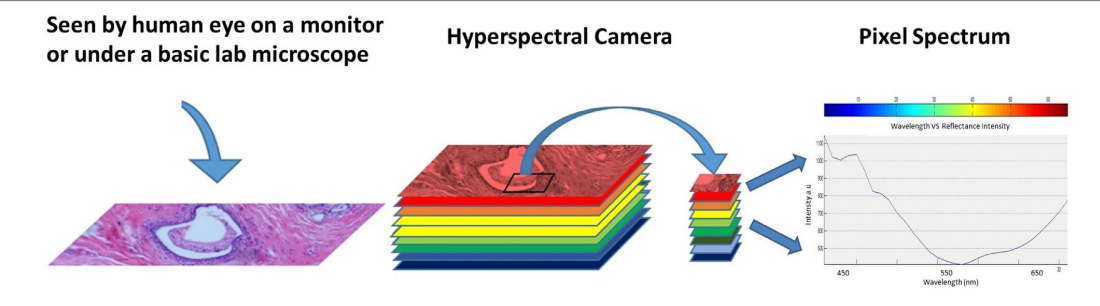
\includegraphics[scale=0.5]{HSI.png}        
        \centering    
        \caption{Hyperspectral image}
        \label{fig:systemArch}
    \end{figure}
       
  
    
  This electromagnetic radiation is not only present among the visible range of wavelengths, as it covers the most part of the electromagnetic spectrum. These kinds of images provide us with useful information as said earlier, as it includes electromagnetic spectrum invisibly to the human eye. However, due to the huge amount of data, processing of HSI images is very computationally expensive.
  
  The experiments of this thesis have been tested using a medical hyperspectral image gathered from the HELICoiD project database. The first illustration displays a dataset of each hyperspectral cube of the brain cancer in RGB,and the second one illustrates the name of each image belonging to the dataset along with their dimensions (rows,columns and bands).
  
  
   \begin{figure}[H]
        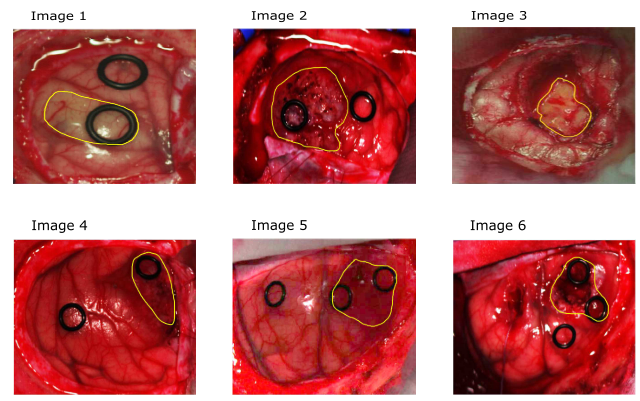
\includegraphics[scale=0.8]{HS_dataset.png}        
        \centering    
        \caption{Brain Cancer dataset}
        \label{fig:systemArch}
    \end{figure}
    
    
   \begin{figure}[H]
        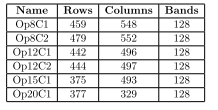
\includegraphics[scale=1.3]{table_dimensions.png}        
        \centering    
        \caption{Dimensions of each image}
        \label{fig:systemArch}
    \end{figure}
     
   \subsection{Applications} 
    Hyperspectral images are mostly used for identifying and estimating different materials within a captured image in the spectral region.
    This technology was initially employed to remote sensing applications, specifically, earth observation and geology. Other than the previously mentioned applications, remote sensing is used in a great variety of applications, such as security and defence, agriculture and food engineering, eye care, mineralogy, surveillance, astronomy... 
    
    
   \subsubsection{Remote Sensing} 

As was mentioned earlier, hyperspectral images are one of the promising remote sensing technology. 

  \subsubsection{Cancer Detection} 

Hyperspectral imaging is a non-contact, non-ionizing and minimally-invasive sensing technique suitable for medicine. It consists in collecting and processing information from across the electromagnetic spectrum creating a hyperspectral image. This kind of images increases the information acquired from a scene compared with a conventional RGB image
Hyperspectral        	
         	
\section{Classifiers}
     
     \subsection{Concept}
      
Image processing consists of a mathematical algorithm that, when applied, derives information from an image that can be used in automated image analysis systems.\cite{khouj2018hyperspectral}. 
 
 	In this context this mathematical algorithm is known as a classifier. The main aim of a classifier is to be able to provide a classification algorithm using observations or data and to train this algorithm based on those data,to finally distinguish at which class belong to.
 
	The process of learning begins with observations or data, such as examples, direct experience, or instruction, in order to look for patterns in data and make better decisions in the future based on the examples that we provide.[pagina web 1] Once the classifier has been trained, it is able to associate any data to a specific class using new input parameters called test dataset. In other words, a classifier is an algorithm that associates the input data to a specific category.
	
	
	The main practical objectives of machine learning consist of generating accurate predictions for unseen items and of designing efficient and robust algorithms to produce these predictions, even for large-scale problems.
	
	
	  \begin{figure}[H]
        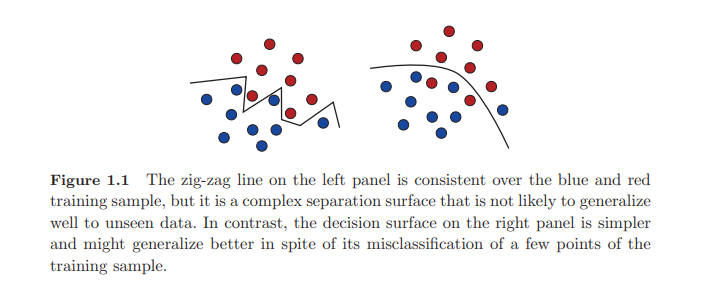
\includegraphics[scale=0.8]{machinelearning.png}        
        \centering    
        \label{fig:systemArch}
    \end{figure}
    
     \subsection{Unsupervised classification}
            
   Input data is not labelled and does not have a known result.

	A model is prepared by deducing structures present in the input data. This may be to extract general rules. It may be through a mathematical process to systematically reduce redundancy, or it may be to organize data by similarity.

	The learner exclusively receives unlabeled training data,and makes predictions for all unseen points. Since in general no labeled example is available in that setting, it can be difficult to quantitatively evaluate the performance of a learner. Clustering and dimensionality reduction are example of unsupervised learning problem\cite{mohri2012foundations}.
	Clustering in its elemental form is defined as a algorithm of identifying homogeneous groups of data points in a given data set.
	The algorithm under study in this master thesis belongs to this kind of classification. This algorithm will be explained in detail later.

    \subsubsection{KMeans} 
                   
K-Means is a learning algorithm used mainly to resolve unsupervised data classification problems. The K-Means algorithm determines k number of centers (one for each cluster),then associate each data point to the nearest centre. 

	It is necessary to define some crucial concepts in order to truly understand this algorithm. A centroid is a data point at the center of a group and each of these groups is called a cluster and is a region in which the density of objects is locally greater than in other zones and share similar features.

	Placing the centroids as far away from each other as can be, when the k centroids are initialized, is the best way of increasing the detection accuracy and minimize the numbers of errors.

 	Furthermore,unsupervised clustering is used to describe processes where a classifier is assigned a dataset without preexisting labels\cite{thomas2002randomized} \cite{kushi2012american}.
 	            
    \subsection{Supervised classification}
            	
The learner receives a set of labeled examples as training data and makes predictions for all unseen points. This is the most common scenario associated with classification, regression, and ranking problems\cite{mohri2012foundations}.

In supervised learning the input data is labeled, which means that each instance of the data set consists of an input vector and a corresponding output value \cite{mohri2012foundations}. A machine learning algorithm solves the problem relying on this label input. The resulting model may be employed for classifying and predicting new unknown data.
	
    \subsection{Processing chain for hyperspectral images}
            
The procedure is as follows; in order to obtain the hyperspectral images of the in- vivo human brain surface during the neurosurgical operations, the HELICoiD project has built a demonstrator capable of simultaneously obtaining two hyperspectral cubes.  

	 A preliminary step called pre-processed is performed in order to decrease the amount of information, such as making a radiometric calibration, reducing the noise and the dimensionality, and finally, normalizing the HS image.Once this preliminary step has been reached, they are analysed using the supervised as well as unsupervised classification.

	In terms of unsupervised classification, HS cubes are clustered employing K-Means, which defines different areas properly, however, they have no meaning. After using this algorithm, an unsupervised segmentation map is generated.Meanwhile in parallel, the system executes a number of algorithms belonging to supervised classification. These algorithms are PCA (Principal Components Analysis), SVM (Support Vector Machine) and KNN (K-Nearest Neighbour). In order to approach real time during surgery, the parallelization of these algorithms is required.

   After performing these algorithms, tissues are displayed using different colours in order to represent the associated classes. 
Applying the majority voting, the unsupervised segmentation map obtained from K-Means clustering algorithm as well as the classification map obtained from supervised classification, are merged. 

	As it can be observed on the image below, the process can be divided into three fundamental parts: the first one belonging to the execution of the PCA and SVM algorithms in parallel. Once it is performed,the process continue with the second part, the implementation of the KNN algorithm. Meanwhile, in parallel with the previous steps (first and second),K-Means is executed.

	  \begin{figure}[H]
        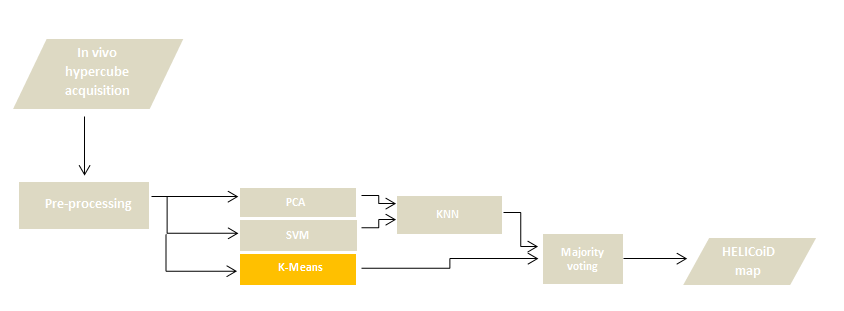
\includegraphics[scale=0.8]{processingchain.png} 
        \caption{HELICoiD processing chain}       
        \centering    
        \label{fig:systemArch}
    \end{figure}
	
	
 	\subsubsection{PCA (Principal Component Analysis)}              
 	\subsubsection{SVN (Support Vector Machine)}
 	\subsubsection{KNN (K-Nearest Neighbor)}

\section{Parameterized and Interfaced Synchronous DataFlow MoC} 
   A wide number of applications within the field of Digital Signal Processing (DSP) such as video decoding, telecommunication and computer vision use Dataflow Models of Computations (MoCs) because of their flexibility, analysability and natural expressivity that ease the parallelization of the applications.
   
   Before going through PiSDF model, we will first define the concept of a Synchronous DataFlow (SDF). SDF is a restricted form of dataflow in which the numbers of tokens produced and consumed by each actor execution are restricted to be constant and statically known (known at compile time)\cite{bhattacharya2001parameterized}.In this kind of model, a graph is used for describing an application in which nodes describe computations and the stream of data-tokens between operations are transmitted by edges. Edges works with initialization tokens called delays as well.
   
   This model called PiSDF extends the semantics of a targeted dataflow MoC and integrates parameterized along with interface-based dataflow. In the case of parameterized dataflow, parameters can have influence on different properties like the firing rules of actors. In the second case,however, predictability is improved since it enables a top-down parametrization and it limits the scope of the parameters. 
   
  Regarding $\pi SDF$ Semantics, a $\pi SDF$ \cite{desnos2013pimm} graph G = (A, F, I, $\Pi$, $\Delta$) contains, in addition to the SDF actor set A and FIFO set F, a set of hierarchical interfaces I, a set of parameters $\Pi$, and a set of parameter dependencies $\Delta$.
   
   \begin{itemize}
   \item Interface-Based Synchronous Dataflow MoC is a hierarchical extension of the SDF model interpreting hierarchy levels as code closures. IBSDF adds interface elements to insulate levels of hierarchy in terms of schedulability analysis \cite{desnos2013pimm}
   
   An example of an IBSDF graph is displayed and explained hereafter:
      
     \begin{figure}[H]
        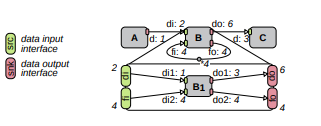
\includegraphics[scale=1]{interfacebsed.png}        
        \centering    
        \caption{Hyperspectral image}
        \label{fig:systemArch}
    \end{figure}
       
A data input interface $i_{data}^{in} \in I_{data}^{in}$ in a subgraph is a vertex transmitting to the subgraph the tokens received by its corresponding data input port. If more tokens are consumed
on a data input interface than the number of tokens received on the corresponding data input port, the data input interface behaves as a circular buffer, producing the same tokens several times.

 A data output interface $i_{data}^{out} \in I_{data}^{out}$ in a subgraph is a vertex transmitting tokens received from the subgraph to its corresponding data output port. If a data output interface
receives too many tokens, it will behave like a circular buffer and output only the last pushed tokens \cite{desnos2013pimm}.

  
   \item Parameterized Dataflow MoCs

Parameterized Dataflow imposes a hierarchy discipline   that incorporates parameterization and run-time management of parameter configurations. Parameters can either be statically defined, or dynamically set by actors at runtime.

As is clearly explained in this paper \cite{bhattacharya2001parameterized},parameterized dataflow modeling framework imposes a hierarchy discipline on an underlying dataflow model and allows subsystem behavior to be controlled by sets of parameters that can be configured dynamically.PSDF can be viewed as an augmentation of the SDF model that comprehensively incorporates parameterization and run-time management of parameter configurations.

\end{itemize}      
         
   \subsection{PREESM} 
      
Nowadays, video coding/decoding or digital communications are applications that are becoming more and more complex and sophisticate. Also, programming architectures such as Digital Signal Processors (DSPs) require high specialization of engineers because of the bottlenecks of the algorithms as well as the architecture, when it comes to implement parallel execution. Therefore, there is a need to implement a more powerful computational models. As was mentioned earlier, the use of parallel architecture may meet requirements.

	To reduce the software development effort for such architectures, it is necessary to provide the programmer with efficient tools capable of automatically solving communications and software partitioning/ scheduling concerns. Most tools such as PeaCE, SynDEx or PREESM use as an entry point a model of the application associated to a model of the architecture\cite{piat2010loop}. The algorithm under study in this work is performed using PREESM.

	PREESM offers great features in terms of memory, time analysis and it has automatic deadlock-free code generation. This tool is an open source rapid prototyping tool. It simulates signal processing applications and generates code for heterogeneous multi/many-core embedded systems. Its dataflow language eases the description of parallel signal processing applications.
	
	Furthermore,PREESM tool inputs are an algorithm graph, an architecture graph, and a scenario which is a set of parameters and constraints that specify the conditions under which the deployment will run. The chosen type of algorithm graph is a parameterized and hierarchical extension of Synchronous Dataflow (SDF) graphs named PiSDF or $\pi SDF$. The architecture graph is named System-Level Architecture Model (S-LAM). From these inputs, PREESM maps and schedules automatically the code over the multiple processing elements and generates multi-core code \cite{pelcat2014preesm}.
	
	
	
	An example of an application graph using PREESM is displayed in figure \ref{fig:graph}.
	
	\begin{figure}[H]
        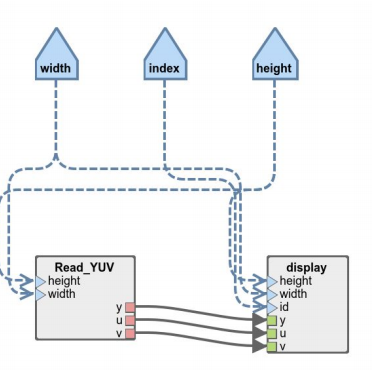
\includegraphics[scale=0.8]{expreesm.png}        
        \centering    
        \caption{Example of application graph \cite{PREESM:2019:Online}}
        \label{fig:graph}
    \end{figure}
	
	This is a typical application graphs that contains the basic components in a network.
	
	Parameters are shown at the upper side, they have impact on the productions and consumption rates of tokens on the data FIFO queues.	
	Actors are entities which are connected each other by First In, First Out data queues (FIFOs). A actor fires when the FIFO have enough incoming tokens. A firing rules set the number of data tokens consumed and produced by an actor.The internal behavior of actors is manually programmed in language supported by the architecture compiler, e.g. C or C++ code.
	
	
	
	
	
	  
  
\chapter{K-Means Clustering Algorithm}
	\label{sec:kmeans_algorithm}
	This present section describes how the design challenges were solved in this project with respect to the serial implementation. Methods and procedures are explained in detail throughout this chapter as well.

    \section{K-Means algorithm for hyperspectral images}
    
    
    In the field of image processing, namely hyperspectral image, the clustering algorithm called K-Means is described as follows:
    
     First, K centroids are defined, one for each cluster (K number of clusters). After initializing these variables, a first grouping is implemented as the distance of each point to the centroids. Each point is identified with a cluster represented by the nearest centroid. A centroid represents the center of a cluster, in order to find it, an average of the data is performed, this refers to the means in the K-Means algorithm. This process is perform iteratively until the difference between centroids of two consecutive iterations is either smaller than a specified error or the maximum fixed number of iterations is reached. 
    
    
    The purpose of executing the processing tool chain during surgery is to define the tumour borders with precision. K-means is the algorithm that best meets this need since the major role is separate clearly different areas of the hyperspectral image. 
    
 For hyperspectral data, the classifier can be used to find spectral classes in a multiband image without assigned values from the data provider. The clustering treats unsupervised data by providing access to the tools to learn the classification from the data itself to create clusters that group the data based on the desired classification\cite{kushi2012american}.
  
 	It should be noted that in contrast with all other algorithms (PCA, SVM and KNN), K-Means does not need prior knowledge of the data; therefore, it does not have a number of fixed steps. Furthermore,data are put together in terms of feature similarity. 
 	
 
 
    \subsection{Analysis of the pseudo-code}
    
The pseudo-code described hereafter (algorithm 1), it has been taken from \cite{torti2018paralle}, where $\gamma$ indicates a hyperspectral image that consists of N pixels and L bands. Therefore, a hyperspectral image is a matrix with size $NxL$. The parameters to be set when it comes to execute the algorithm are as follows: 
\begin{itemize}
\item K which corresponds with the number of clusters to use.
\item $Min\_error$ related to the minimum error allowed.
\item $Max\_iter$ are the maximum number of iterations which are executed.
\end{itemize}

 \begin{figure}[H]
        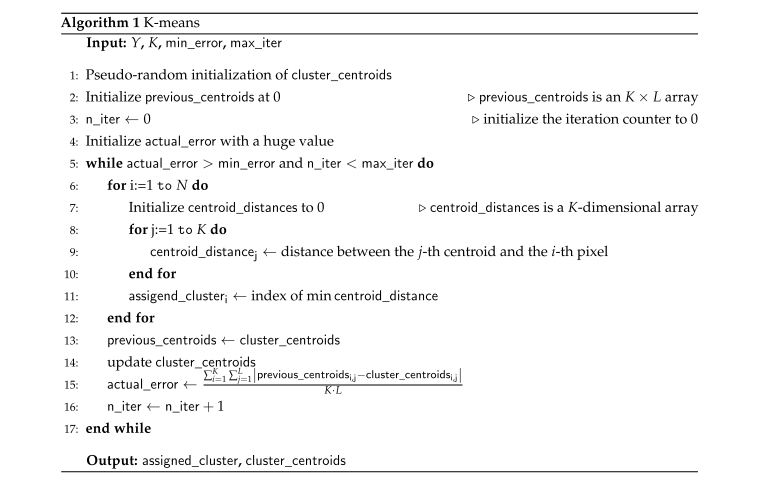
\includegraphics[scale=0.8]{pseudocode.png} 
        \centering   
        \caption{Pseudo-code of the K-means   \cite{torti2018paralle}}        
        \label{fig:systemArch}
    \end{figure}

The k-means algorithm generates different results. On one hand, a $KxL$ array including the centroids, which is called $cluster\_centroids$ and an $N-dimensional$ array which has the label of the cluster assigned to each pixel, this parameter, by contrast, it is called $assigned\_cluster$.

The K-means clustering algorithm is analysed in detail line by line. First,in lines 1 and 2 the initialization of the variables is perform. Namely,
$cluster\_centroids$ is initialized with K different hyperspectral pixels pseudo-randomly taken from the input image $\gamma$.

 The variable $actual\_error$ is initialized with a great value to make sure that the main loop is executed at least one time.
 
 As can be seen in the figure above, there are two iterative loops (from lines 6 to 12), the inner one is executed K times which are the number of clusters, and the external one iterates over the number of pixels N, instead. 
 
  A temporal array determined by $centroid\_distances$ is set to 0 and it stores the distances between each pixel and the centroids. Spectral Angle (SA) formula is used in order to calculate the measured distance between them.
  
  This Spectral Angle is defined as: 
 
   \begin{figure}[H]
        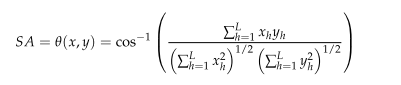
\includegraphics[scale=0.8]{Spectralformula.png} 
        \centering  
        \caption{Spectral Angle formula\cite{torti2018paralle}}          
        \label{fig:systemArch}
    \end{figure}
   
 	This formula results in spectral vectors determined by x and y. The variables $x_h$ and $y_h$ are the response of the h-th band of x and y and they go from 1 to L bands.
  
  Once this step has been executed, the label assigned to each pixel corresponds to the group represented by the centroid with the minimum SA value. This step is performed for each pixel. 

After these steps,the array $previous\_centroids$ stores the centroids with the SAs computation, and subsequently, the centroids are updated by calculating the mean value, for each band, of the pixels belonging to the group or cluster. In order to compute the error, $previous\_centroids$ and the updated centroids already calculated, are used for calculating the variation. This value represents how different they are among them, or, how much they have varied in each iteration. In addition, it is used as a stop condition when this difference is smaller than a fixed threshold ($actual\_error)$. The number of iterations is increased in each iteration, and when it reaches a value (threshold) which has been set previously,the algorithm is no longer executed. 

     \subsection{C serial code profiling}
     
	As was mentioned earlier, the C serial code has been provided by Universidad de Las Palmas de Gran Canaria.  This algorithm has been analysed in detail in order to do a  first approach of how it works internally and how each function was implemented, and then be able to parallelize it. A dataset of real HS images is used for the processing toolchain. Before executing this algorithm, certain parameters may be set, these parameters are as follows:
	
	$$K=24$$
	$$min\_error=1\mathrm{e}{-3}$$
	$$max\_error=50 \thinspace iterations$$
	
	All these parameters have been taken from \cite{torti2018paralle}. The K value was set during the development of the HS brain cancer algorithm illustrated in \cite{fabelo2018spatio}.If this configuration is set, the algorithm never reached the maximum number of iterations established.
	
	It should be noted that a function in C has been created by each process described previously. As the purpose of this research work is to parallelize a clustering algorithm, the C serial code has to be analysed in depth in order to study the heaviest part and the bottlenecks of the code which slow down the algorithm and does not allow to approach real time, which is crucial for neurosurgeons during surgery.
	
	The heaviest part of the code is undoubtedly the computation of distances,as was mentioned earlier, is the spectral angle between each hyperspectral pixel and the centroids. The time invested in the computation of the distance is approximately 26 seconds (based on the serial implementation), which along with the other functions executed inside the loop, take the 94$\%$ and $98\%$ of the time for the smallest and the biggest image according to this paper \cite{torti2018paralle}.
	
	Furthermore, initialization functions such as initialization of the error and initializaton of $cluster\_centroids$ are not parallelized since they are executed just one time in the beginning and they are not a point for consideration. 
	
	
	 \subsection{K-means in PREESM}
	 
	 The algorithm has been first implemented using $\pi SDF$ dataflow model in PREESM in order to ensures consistency and schedulability and then parallelised
	 	 
	As was explained earlier,the  $\pi SDF$ MoC is a generalization of the SDF MoC.In addition to the actors and FIFOs of the SDF semantics, the  $\pi SDF$ semantics has a set of parameters and parameter dependencies that can be used to reconfigure the production and consumption token rates of actors. Furthermore, the  $\pi SDF$ semantics has a hierarchy mechanism that enables the composition of graphs by using a $\pi    SDF$ sub-graph as a specification of the internal behaviour of an actor.
	
	First of all, the algorithm has been divided into different hierarchies in order to create independent graphs that isolate themselves from each other. Its behaviour (the instantiated ones) may not be modified by its parent graph.
	
	As this kind of model allows to create different hierarchies, a top diagram is first created. This hierarchy includes three main actors known as, "read parameters", "kmeans cluster" and "write parameters" which are explained in detail as follows:
	
	\textbf{Read parameters's actor}: A whole hyperspectral image is read and stored by this actor, from either a binary file or txt file in order to process it. Each token corresponds to a pixel in a particular band.
	 Furthermore, this actor reads a parameter called par which is the minimum error allowed.
\par
	\setlength\parindent{24pt}\textbf{Kmeans cluster}: A whole image is processed by one firing of kmeans cluster actor. This actor is refined by several actors such as initialize cluster, initialize error and kmeans function. Kmeans function actor is a hierarchical actor defined by the subgraph  formed by actors loop, compute error, compute distance and update centroids. \par
	\setlength\parindent{24pt}\textbf{Write results's actor}: This actor converts results to a image. The result is a clustered hyperspectral image.
	
	
	 \begin{figure}[H]
        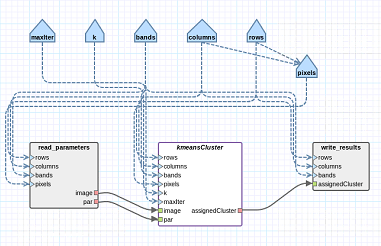
\includegraphics[scale=1.2]{top_diagram.png} 
        \centering 
        \caption{Top PiSDF graph}         
        \label{fig:systemArch}
    \end{figure}
	
	 
KmeansCluster's actor is a hierarchical actor formed by initialize cluster,initialize error and kmeansfunction. A detailed explanation is given hereunder:


\setlength\parindent{24pt}\textbf{Initialize cluster centroids}: This actor assigns an initial value to the centroids: k random non-repeated numbers are taken as indices; 
pixels of the provided set of images corresponding to these indices are the first centroids of the clusters.

\setlength\parindent{24pt}\textbf{Initialize error}: This actor calculates error between current and previous centroids. It should be noted that the error is the mean of the absolute value of the member-to-member difference of the two vectors.

\setlength\parindent{24pt}\textbf{Kmeansfunction}: This is a hierarchical actor set by loop, compute error, compute distance and update centroids actors. They will be explained later.

Finally, the deeper sub graph consists of various actors called loop, compute error, compute distance and update centroids.

\setlength\parindent{24pt}\textbf{Loop}: This actor allows create an iterative loop among actors. Actor loop is used to set the number N of iterations of the for loop.

\setlength\parindent{24pt}\textbf{Compute error}: This actor has the same behavior as the initialize error one explained earlier.

\setlength\parindent{24pt}\textbf{Compute distance}: This actor calculates the distance between each pixel and the centroids of the clusters. Each pixel is assigned to the nearest cluster. The spectral angle is used for computing the distance.

\setlength\parindent{24pt}\textbf{Update centroids}: This actor updates the centroids. In order to get an updated version of the centroids, they are calculated as mean of the elements of the cluster.


   Before starting parallelizing, the whole $\pi SDF$ graph has been tested with the hyperspectral dataset already used for serial code. The obtained clustering is the same as it was obtained in the serial implementation. This has been proven setting a fixed value in the initialization of the cluster centroids (the first cluster centroids are usually selected randomly) and analysing if the image obtained is equal to the achieved by the serial code. The parallelization of the algorithm is performed since the result turned out to be equal to the serial implementation.




	 
	
	
	
	


\chapter{Parallel Implementation}
	\label{sec:parallel_implementation}
	This section describes how the parallelization of the algorithm has been implemented. Furthermore, bottlenecks are studied in detail since they are the ones which cause the greatest delays in the algorithm.

    \section{Parallel K-Means implementation}
    
  The K-Means clustering algorithm has been designed and implemented using $\pi SDF$ dataflow model since it provides flexibility and analysability. The PiSDF dataflow model is used to  algorithms
aims at providing coarse grain parallel descriptions of algorithms specifying precisely the data flowing between actors
and offering a tradeoff between dynamic behavior and predictability.
   So far, both the pseudo code and the $\pi SDF$ graph of the algorithm have been described, the next step is to start the analysis of what is parallelizable. In order to do it achievable, the execution times of each method is calculated and analysed since there are some of them that take most of the clustering algorithm execution time. The first approach will be explained below, and this implementation includes the heaviest operation  which is called compute distances, and if successful the processing time will be reduced dramatically.
  
   \begin{table}[h!]
  \begin{center}
    \begin{tabular}{l|c|r}
      \textbf{Operation} & \textbf{Time(s)}\\
      \hline 
      Operation 1: Initialize centroids & 0.620\\
      Operation 2: Compute error & 0.000023\\
      Operation 3: Compute distance and find minimum & 13.682\\
      Operation 4: Update centroids & 1.056\\
    \end{tabular}
\caption{Individual execution times}
  \end{center}
\label{tab:template}
\end{table}


Table \ref{tab:template} illustrates above-mentioned analysis.As shown, there is one operation that consumes more than the 91$\%$ of the global K-means processing time: the computation of the distances between every pixel and the centroids. Therefore, this computation will be the first to have been parallelized in order to achieve a great time reduction in the algorithm.

   \subsection{Parallel versions of the K-means algorithm}
\begin{enumerate}[label=\textbf{\arabic*})]
   \item \textbf {Parallelization of the computation of the distances} \newline
    The heaviest part of the code is the computation of the distances, which are calculated among pixels and centroids. The computation of the distance can be implemented in parallel since there is no data dependency with the evaluation of a particular pixel and the others.
   
   The first parallel version of the K-means algorithm is based on the parallelization of the distance computation. In this first approach each thread performs the computation of the distance between a particular pixel and the k centroids. This function has been first parallelized since this is one of computations that takes more time.

 \item \textbf {Parallelization of the computation of the distances and find the index of the minimum distance} \newline
   The computation of the distances is parallelized as well as the search for the minimum distance. Since the distances are stored in an $NxK array$, N threads are used for finding the index of the minimum distance. The for loop is performed by the i-threads which compute the operation of the minimum distance. 

\item \textbf{Parallelization of the computation of the distances, find the index of the minimum distance and update centroids} \newline
  The update centroids has been parallelized along with the computation of the distance and the search of the minimum distance. This task has been parallelized by assigning to each thread the computation of the update of the centroids. In other words, each thread is responsible for the update of the assigned centroids.
\end{enumerate}   
   

     	\subsubsection{Bottlenecks}
     	
        \subsection{PREESM implementation}
   Preesm is a dataflow language which aims at easing the description of parallel signal processing applications.
   The aim of this section is to alter the original PiSDF dataflow model of the K-Means application in order to expose a parameterizable degree of data parallelism.
   
   \begin{center}
   \textbf{Computate distance actor}
    \end{center}
   The previous analysis of the execution's times has illustrated that this operation consumes almost a 92$\%$ of the global execution time of the K-means algorithm. 
    
           After executing the workflow on the dual-core scenario, a PiSDF graph is generated. It can be generated the SRDAG with equal productions and consumptions rate from the .pi graph. As can be seen, the graph illustrates 2 duplicates of compute distance actor, each responsible for the computation of the spectral distance between each pixels and the k centroids. This graph is  displayed as follows:  

\chapter{Experimental Results and Discussion}
	\label{sec:results}
	The evaluation of the project was performed in three steps - verification, validation, and benchmarking. 
The following subsections describe each of the steps in details.
    \section{Accuracy analysis}
    \section{Timing analysis}
   
\chapter{Conclusion}
	\label{sec:conclusion}
	This chapter summarizes the work done in this project. 
It reviews if the goals were achieved, presents the main areas of future work, and provides final reflections.
\section{Goals Achieved}
    
\section{Future Work}
    
\section{Reflections}



\printbibliography
%\bibliographystyle{plain}
%\bibliography{bibl}
\end{document}
